% This conference manuscript template is prepared for:   
% Kim Stockment, Conference Coordinator, Ray W. Herrick Laboratories, Purdue University, West Lafayette, IN, USA. 
% Latest revision = 2016-02-23 

\documentclass[10pt]{article}
% Miktex users: require l3 packages
%             : optional 3 packages
\usepackage{multicol,titlesec,apacite,tabto, multirow, makecell}
%\usepackage[round]{natbib}  
\usepackage{longtable}

\usepackage[hmargin = 1in, vmargin = 1in]{geometry}

\renewcommand{\refname}{References}
    
%\usepackage[MnSymbol]{mathspec}
%\setallmainfonts{Times New Roman}
% Mathspec requires the XeTeX compiler. 


\usepackage{lineno,hyperref}
\modulolinenumbers[5]

\usepackage[T1]{fontenc}
\usepackage[utf8]{inputenc}
\usepackage{textcomp}
\usepackage{gensymb}
%%-- mwetter. \usepackage{multicol}
\usepackage{nopageno}
\usepackage{times}
\usepackage{natbib}
\usepackage{enumitem}
\usepackage[font=it]{caption}
\usepackage{doi,url}
\usepackage{hyperref}
\usepackage[usenames,dvipsnames]{xcolor}
\usepackage{listings}
\usepackage{booktabs}
\usepackage{array}
\usepackage{placeins}

%----------------------------------------------------------------%
%              Math                                              %
%----------------------------------------------------------------%

% \usepackage[linesnumbered, ruled]{algorithm2e}
\usepackage{algorithmicx}
\usepackage{algorithm}% http://ctan.org/pkg/algorithm
\usepackage{algpseudocode}% http://ctan.org/pkg/algorithmicx
\renewcommand{\algorithmicrequire}{\textbf{INPUT:}}
\renewcommand{\algorithmicensure}{\textbf{OUTPUT:}}
\renewcommand{\algorithmicforall}{\textbf{for each}}

\usepackage{siunitx}
\usepackage{amsmath}
\usepackage{amsfonts}
\usepackage{amssymb}
\usepackage{mathtools}
\usepackage{eurosym, booktabs, units}
% \usepackage[top=2.5cm, bottom=2.5cm, left=1.5cm, right=1.5cm,
% columnsep=0.8cm]{geometry}
\usepackage{setspace}
\usepackage{fancyvrb}
\usepackage{psfrag}


%----------------------------------------------------------------%
%   FLOATS, FIGURES, TABLES, TYPOS                               %
%----------------------------------------------------------------%
\usepackage{xtab}
\usepackage{verbatim}
% \input{tikz_pck}  % TikZ graphics
% defines lengths for figure plotting
\newlength\figureheight
\newlength\figurewidth
\usepackage{tikz,pgfplots}
% \usepackage{epsfig}
\usepackage{epstopdf}
\usepackage{graphicx}
\usepackage{caption}
\usepackage{subcaption}
\usepackage{color} 
\definecolor{DarkBlue}{rgb}{0.00,0.00,0.55}
\definecolor{DarkGreen}{rgb}{0.050,0.5,0.053}

\setlength{\abovecaptionskip}{0.2cm}
\setlength{\belowcaptionskip}{0cm}
\setlength{\parindent}{0pt}

%%%% Typing commands %%%%
\newcommand{\freg}{f_{\Theta}}
\newcommand{\mbbox}{\ensuremath{\rule{0pt}{0pt}\hfill
    \text{{\scriptsize $\blacksquare$}}}}
\newcommand{\mwbox}{\ensuremath{\rule{0pt}{0pt}\hfill
    \text{{\scriptsize $\square$}}}} 
\DeclarePairedDelimiter{\abs}{\lvert}{\rvert}
% MPC formulation
\newcommand{\lrp}[1]{\ensuremath{\left( #1 \right)}}
\newcommand{\QQ}[1]{Q_{\text{#1}}}
\newcommand{\phm}{\phantom{-}}

\newtheorem{remark}{Remark}

\usepackage{changepage}  % allows to use adjustwidth

\usepackage{titlesec} 
%\titleformat{command}[shape]{format}{label}{sep}{before}[after]
\titleformat{\section}[hang]{\fontsize{12pt}{1em}\selectfont \bfseries}{\thesection. }{0pt}{\centering \MakeUppercase}
\titleformat{\subsection}[hang]{\fontsize{11pt}{1em}\selectfont \bfseries}{\thesubsection}{5pt}{}
\titleformat{\subsubsection}[runin]{}{\thesubsubsection}{5pt}{} 
%\titlespacing{command}{left}{beforesep}{aftersep}[right]
\titlespacing{\section}{0pt}{10pt}{10pt}
\titlespacing{\subsection}{0pt}{10pt}{0pt}
\titlespacing{\subsubsection}{0pt}{10pt}{0pt}	
%\setlength{\bibsep}{3pt}
%\pagenumbering{\gobble}
%\setlength{\hyphenpenalty}{1000}
%\setlength{\exhyphenpenalty}{1000}

\usepackage{fancyhdr}
\pagestyle{fancy}
\fancyhead[R]{\fontsize{12pt}{1em}\selectfont {{\textbf{Page \thepage}}}}
\fancyhead[L]{}
\fancyfoot[C]{IBPSA Project 1}
\renewcommand{\headrulewidth}{0pt} % Turn off the bar

\newcommand\thefontsize[1]{{#1 The current font size is: \f@size pt\par}}


% % % % % % % % % % % % % %  TITLE  % % % % % % % % % % % % % %

\title{MPC formulation description template -- An example}


\author{J\'an Drgo\v{n}a$^{1,2}$}
\date{ ${1}$ Department of Mechanical Engineering,  KU Leuven, Belgium \\
        {\tt\small jan.drgona@kuleuven.be}  \\
            {${2}$ Pacific Northwest National Laboratory, Richland, WA, USA \\
        {\tt\small jan.drgona@pnnl.gov}} \\%
        \vspace{0.2cm}
    \today
}

% \author{J\'an Drgo\v{n}a 
% \thanks{Pacific Northwest National Laboratory, Richland, WA, USA
%         {\tt\small jan.drgona@pnnl.gov}} \
% \thanks{Department of Mechanical Engineering,  KU Leuven, Belgium
%         {\tt\small jan.drgona@kuleuven.be}}%
% }

\begin{document}
	
% \begin{center}
% \vspace{0.2in}
% \noindent{\fontsize{14pt}{1em}\selectfont \textbf{MPC formulation description template -- An example}}\\[14pt]
% 
% {\fontsize{11pt}{1.2em}\selectfont
%  J\'an Drgo\v na\textsuperscript{1}
% \\[11pt]
% 
% KU Leuven\\
% Thermal Systems Simulation  (The SySi) research group  \\[11pt]
% 
% jan.drgona@kuleuven.be\textsuperscript{1}\\
% }
% \end{center}


\maketitle
\thispagestyle{empty}
\pagestyle{empty}

\section*{Abstract}

This document presents an example of the MPC formulation, using IBPSA Project 1 template.
Twelve-zone office building is used for demonstation of the methodology.
% General description of the building is followed by definition of key performance indicators (KPIs) and physical constraints.
Equivalence of MPC formulations using physical notation and control engineering notation is demonstrated using translation template.

% \section{Building Description}\label{sec:building}
% Building envelope and HVAC.
% % 
% \begin{figure}[htbp]
% \centering
% 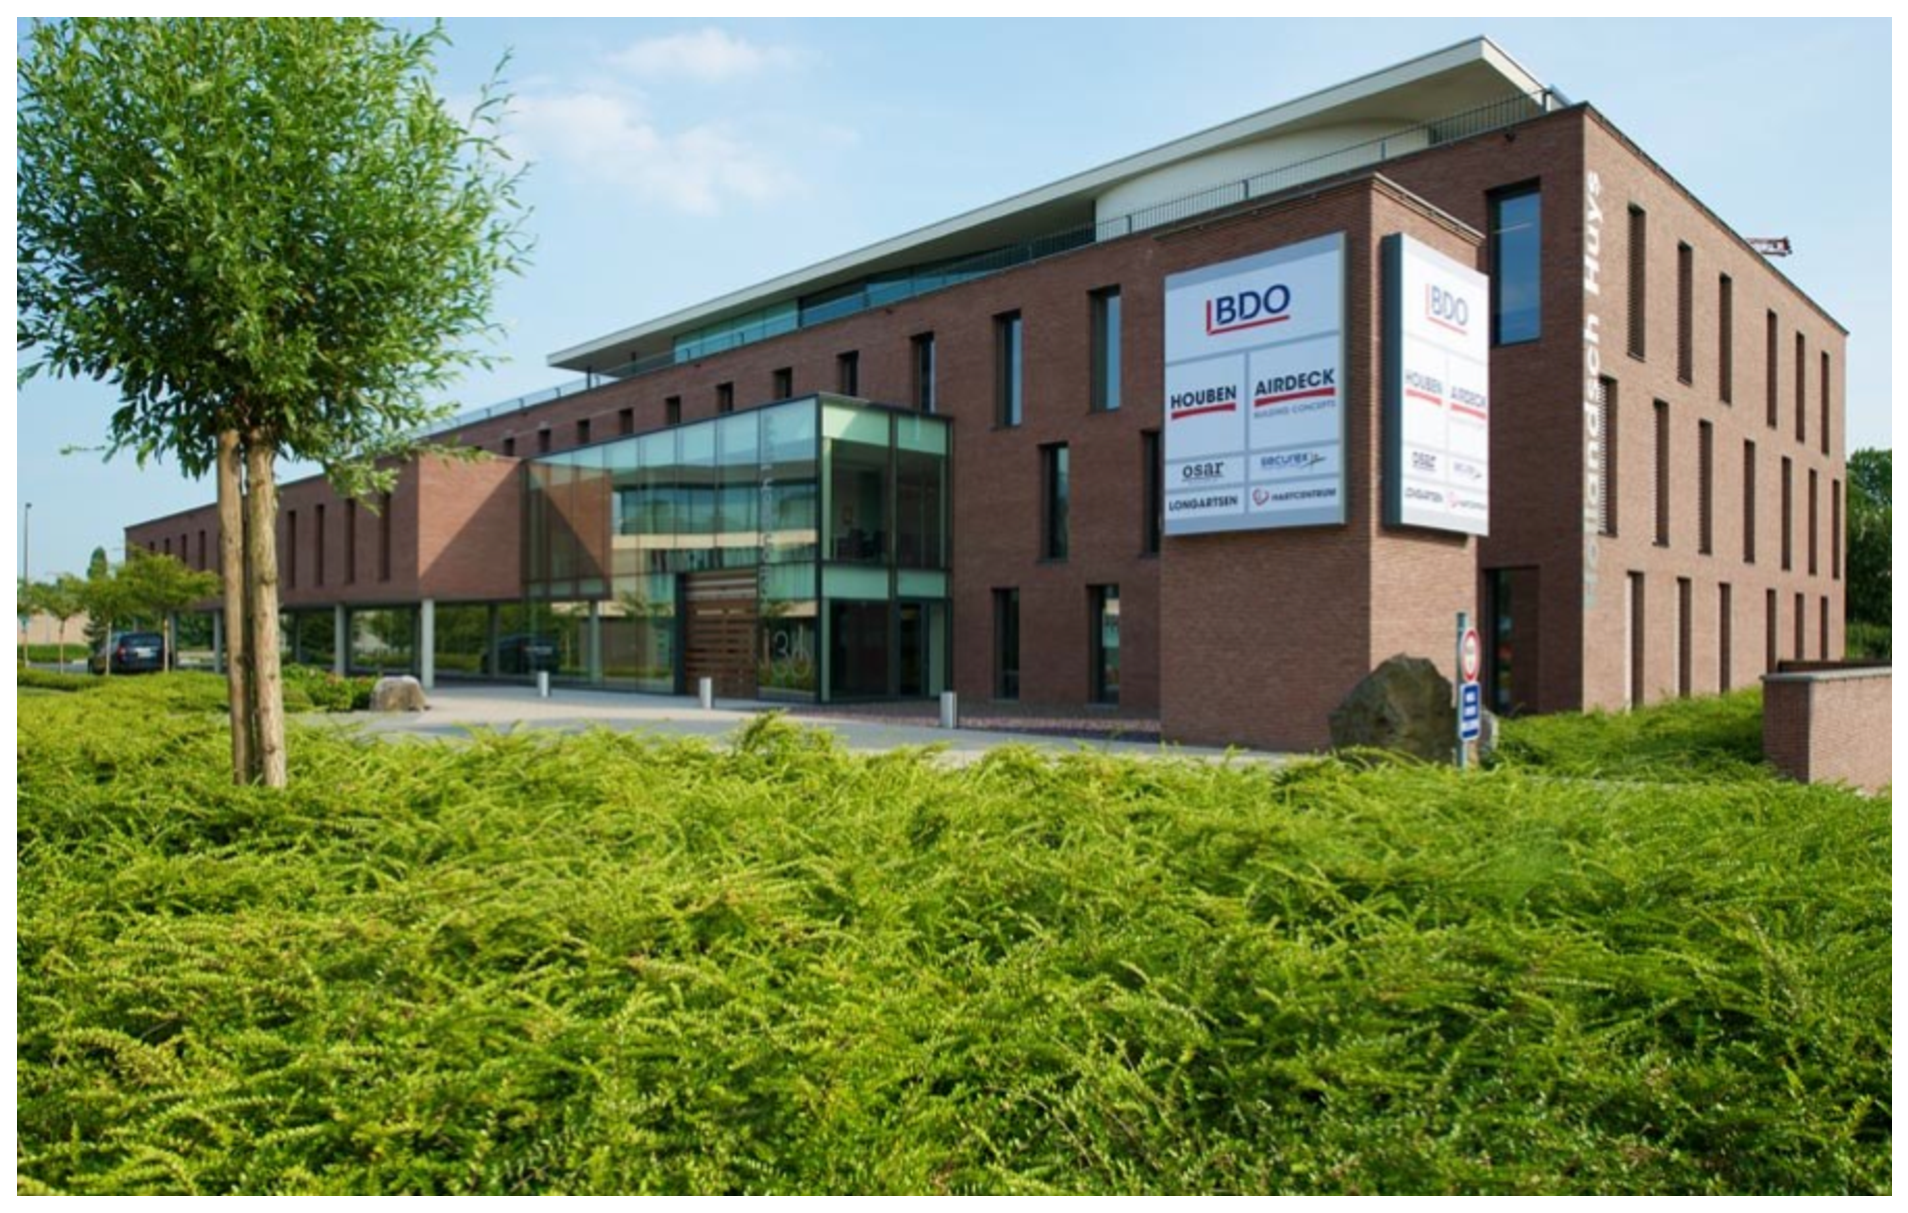
\includegraphics[width=0.80 \textwidth]{fig/HH_building.eps}
% \caption{Hollandsch Huys office building.
% }
% \label{fig:approxMPC:TDNN}
% \end{figure}
% %
% \begin{figure}[htbp]
% \centering
% 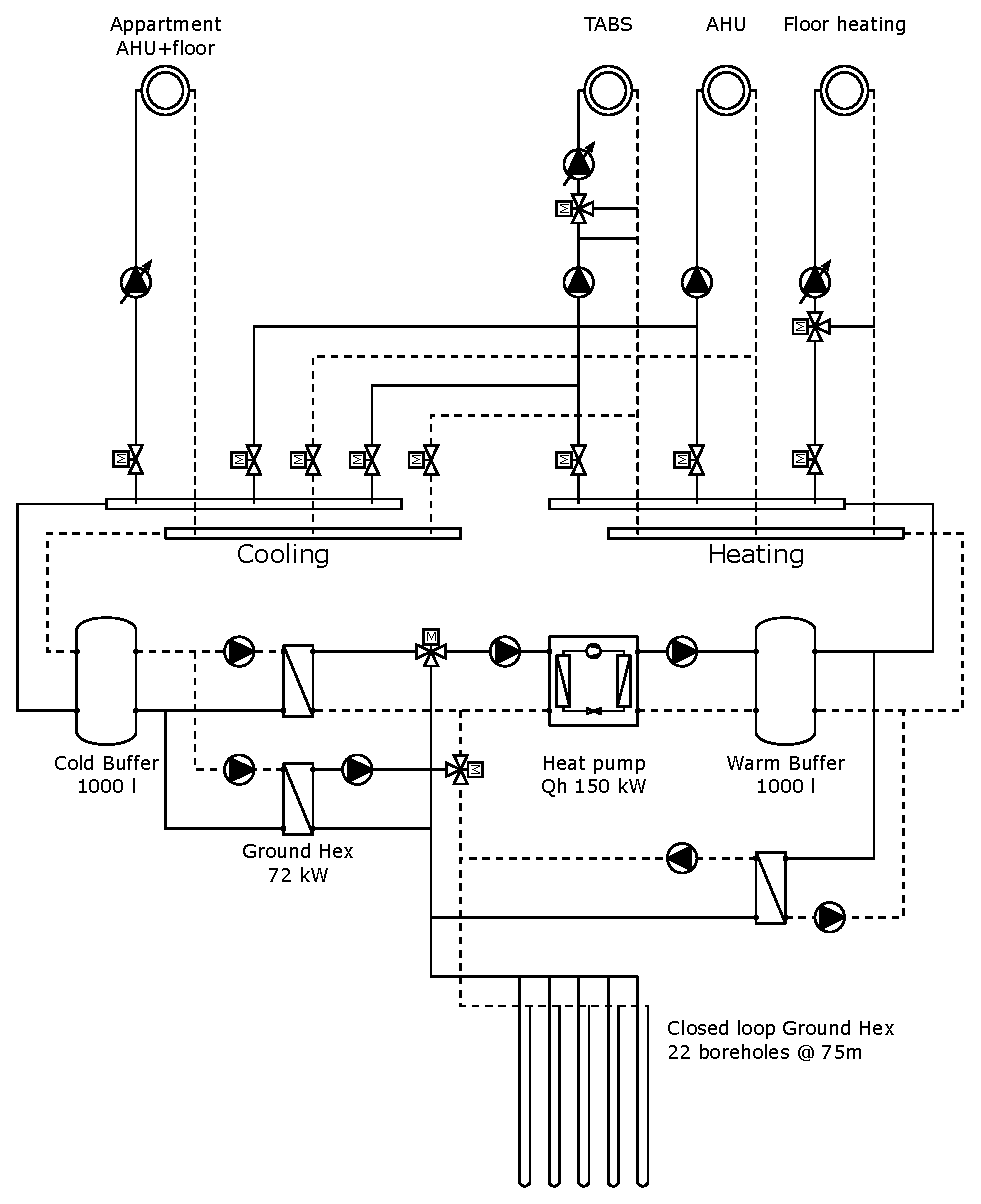
\includegraphics[width=0.80 \textwidth]{fig/HH_HVAC.eps}
% \caption{Hollandsch Huys heating system scheme.
% }
% \label{fig:approxMPC:TDNN}
% \end{figure}


\section{Office Building} \label{sec:building}

% Hollandsch Huys
% 

This section  provides a high-level  overview  of the building and its systems. 
This section is based  on prior modeling work done by Picard~\cite{PicardPhD2018}.
The case study office building shown in Fig.~\ref{fig:HH:HH_building}, called \textit{Hollandsch Huys}, is located in Hasselt, Belgium. 
Its construction was finished in 2007 and it was designed to be a low-energy, innovative 
building.  
% hybrid \textit{GEOTABS} 
% That means the building is equipped with ground source heat pump (GSHP) production system with a gas boiler as a backup system and the main emission system of the building are thermally activated building structures (TABS) and the floor heating.
% 
Fig.~\ref{fig:HH:layout} shows the building's layout, which consists of five floors:  underground parking, three floors, and a roof apartment. 
The following sections describe the building envelope,
the HVAC system, the control oriented model,  the occupancy, internal gains, comfort bounds assumed and RBC.
\begin{figure}[!htbp]
    \centering
    \begin{subfigure}[b]{0.40\textwidth}
        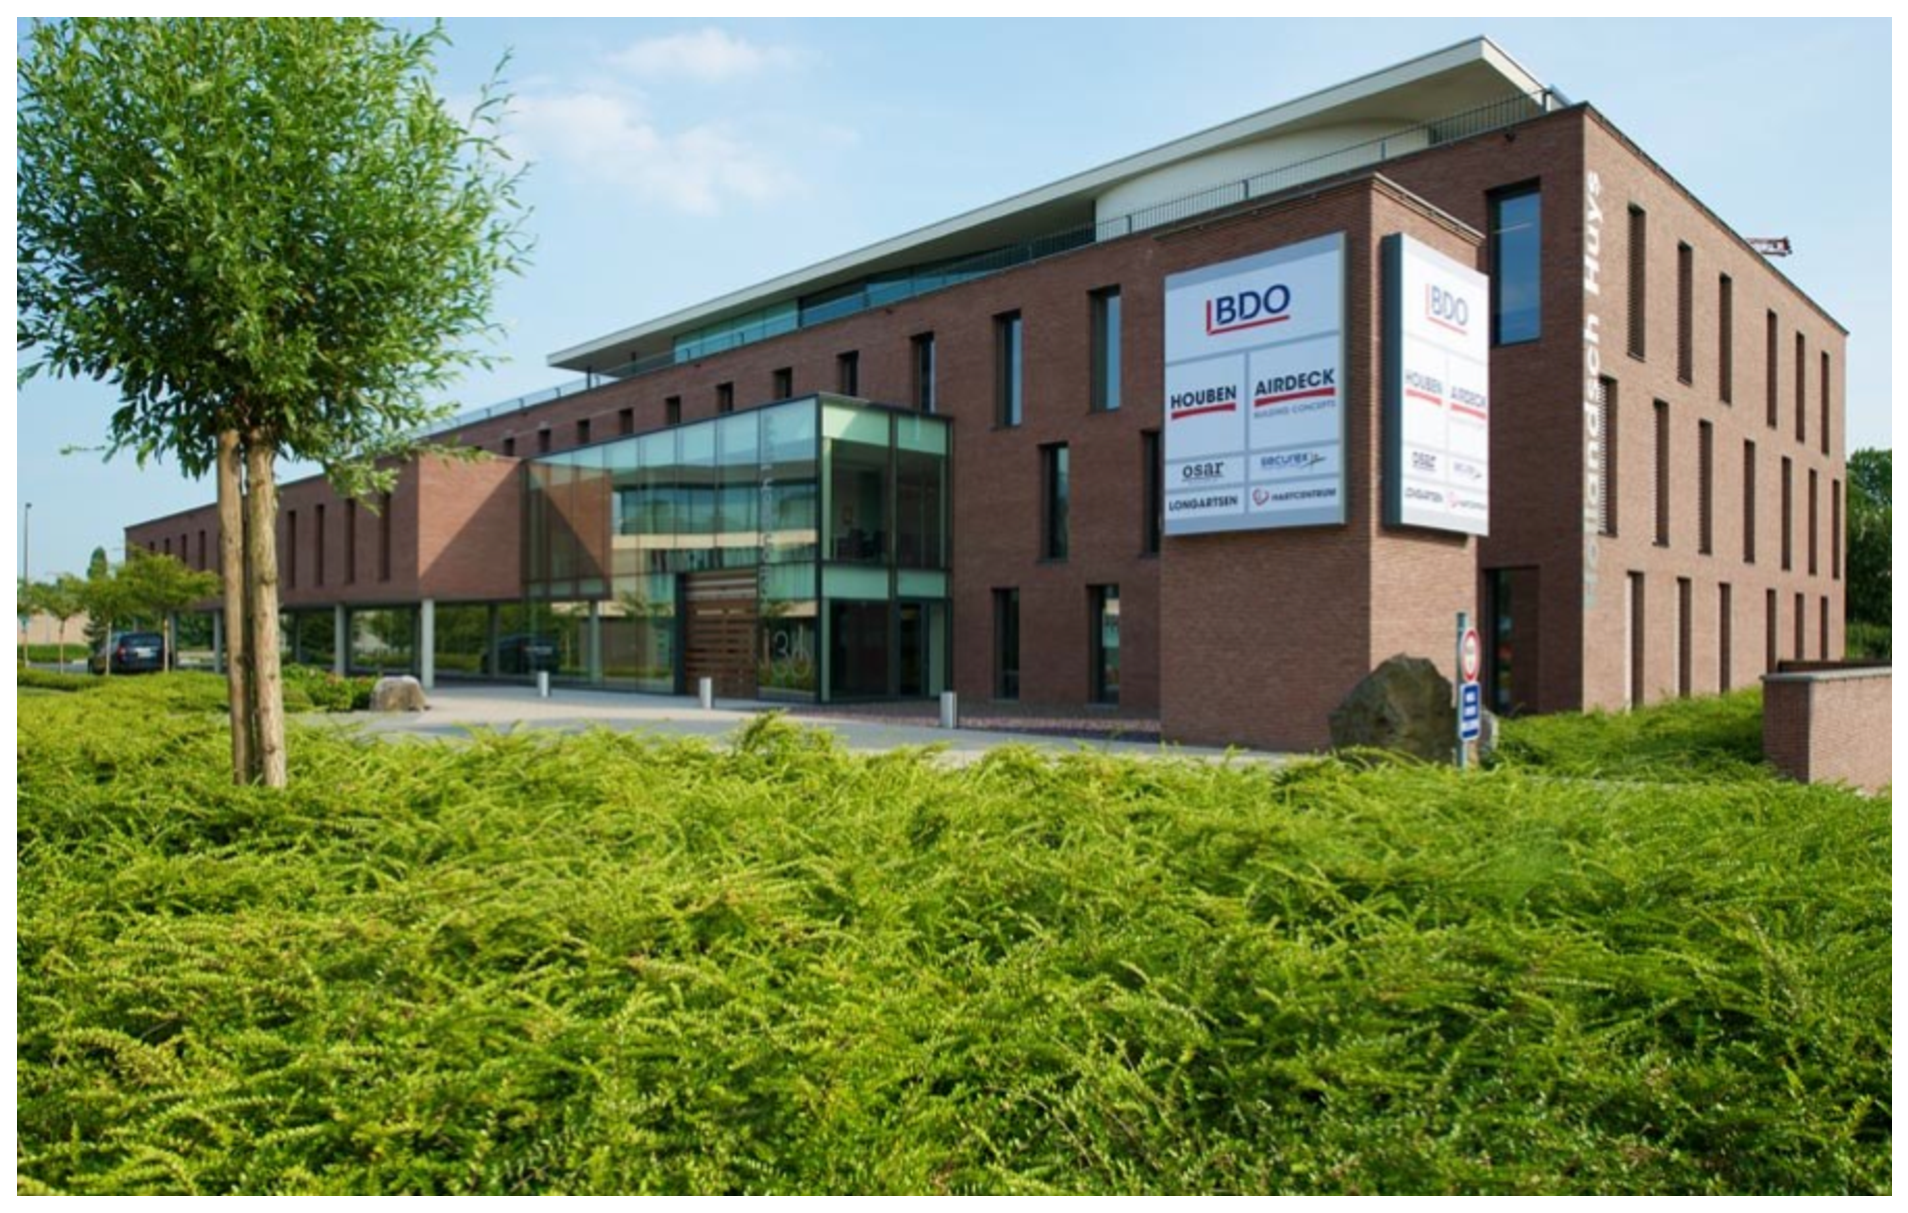
\includegraphics[width=0.85 \textwidth]{fig/HH_building.eps}
\caption{Building from outside.}
        \label{fig:HH:HH_building}
    \end{subfigure}
    ~ %add desired spacing between images, e. g. ~, \quad, \qquad, \hfill etc. 
    %(or a blank line to force the subfigure onto a new line)
    \begin{subfigure}[b]{0.58\textwidth}
        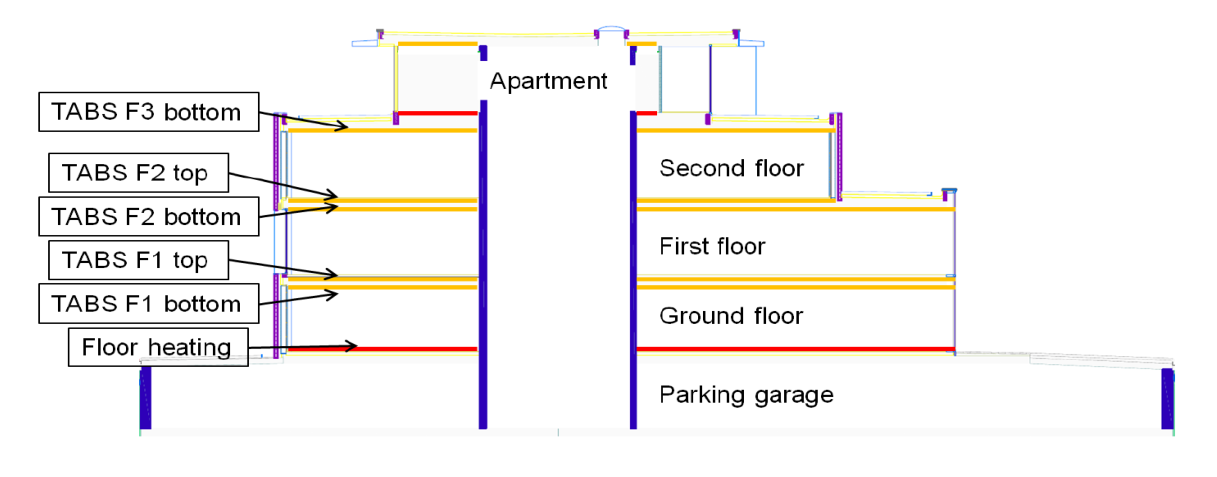
\includegraphics[width=1.00 \textwidth]{fig/HH_layout.eps}
        \caption{Building's layout.}
        \label{fig:HH:layout}
    \end{subfigure}
      \caption{Hollandsch Huys office building~\cite{Zacekova2013Ifmb}.}
    \label{fig:HH}
\end{figure}



\subsection{Building Envelope} \label{sec:building:envelope}

The general parameters of the building envelope are summarized in Tab.~\ref{hh:tab:buiPar}.
The U-value is an average value for the
  whole building and ACH stands
  for \textit{air changes per hour}.
The building is divided into $12$ thermal zones, $4$ per  floor. 
% as depicted by Fig.~\ref{hh:fig:zonLay}.
All transparent parts of the fa\c{c}ade are equipped with triple glazing. 
The window surface lies \SI{40}{\cm} deeper than the
fa\c{c}ade. Each of them is equipped with an external slat shading device 
whose angle is adjusted automatically to the
solar radiation intensity: the shading device is controlled
by a hysteresis controller which closes the shading when the
horizontal solar radiation exceeds \SI{150}{\watt\per\metre\squared}  and re-opens it
when the solar radiation is lower than \SI{80}{\watt\per\metre\squared}.
% 
\begin{table}[!htbp]
  \centering
  \caption{General building parameters~\cite{PicardPhD2018}.
  }
    \begin{tabular}{r|r|r|r|r|r}
    \toprule
    Floor area & [\SI{}{\metre\squared}]  & 3760     & U-value & 
[\SI{}{\watt\per\metre\squared\per\kelvin}] & 0.216 \\
    Conditioned volume & [\SI{}{\cubic\metre}]  & 10526   &  Loss area & [\SI{}{\metre\squared}] & 4438\\
    Window-to-wall ratio & [-]   & 34\SI{}{\percent}   & ACH (n50) & [\SI{}{\per\hour}] & 0.9 \\ 
    \bottomrule
  \end{tabular}%
  \label{hh:tab:buiPar}%
\end{table}%
% 
% \begin{figure}[!htbp]
%   \centering
%   \medskip
% \includegraphics[width=0.7 \textwidth]{fig/zonLay.eps}
%   \caption{Hollandsch Huys zone layout~\cite{PicardPhD2018}.}
%   \label{hh:fig:zonLay}
% \end{figure}


\subsection{Heating Ventilation and Air Conditioning System} \label{sec:building:HVAC}

% % Fig.~\ref{fig:HH_HVAC_overall} shows a general HVAC system overview.
% Hollandsch Huys represents so-called \textit{hybrid} \textit{GEOTABS} building with  emission system 
% composed of thermally  activated building structures (TABS),
%  floor heating, and   air handling  units (AHU).
% The production system is a ground source heat pump (GSHP) 
% and a gas boiler  (GB). 
% The air handing unit (AHU) is composed of a recovery wheel which can be by-passed,
% a heating and a cooling coil and the supply and extraction fans are 
% on-off controlled.
% 
% \begin{figure}[!htbp]
% \centering
% \includegraphics[width=0.70 \textwidth]{fig/HH_HVAC_overall.eps}
% \caption{Hollandsch Huys HVAC system overview.
% }
% \label{fig:HH_HVAC_overall}
% \end{figure}
% \subsubsection{Heat/Cold Production and Emission System} \label{sec:building:HVAC:HC}
Fig.~\ref{fig:HH_HVAC} shows the hydraulic scheme of the building.
\begin{figure}[!htbp]
\centering
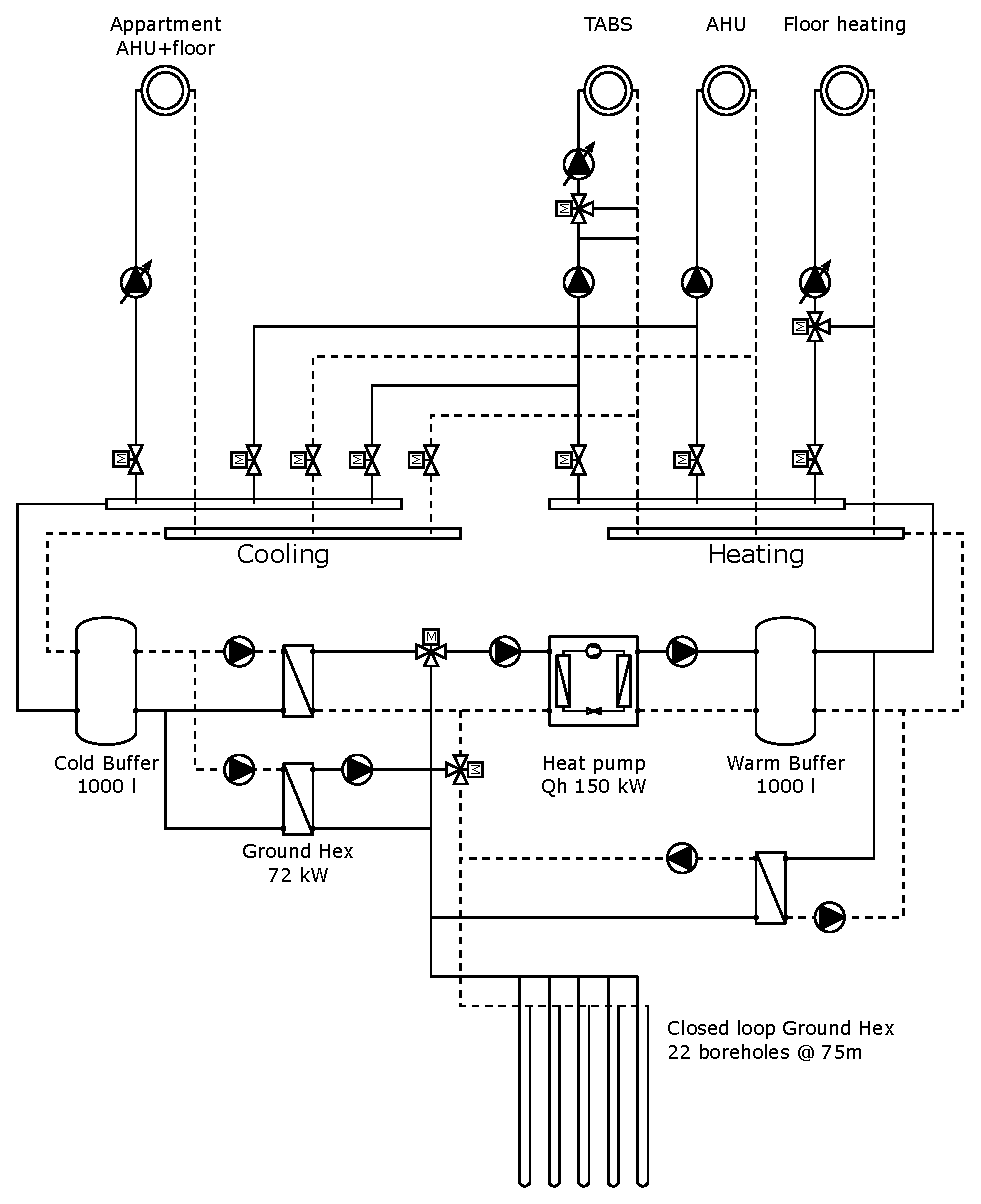
\includegraphics[width=0.50 \textwidth]{fig/HH_HVAC.eps}
\caption{Hollandsch Huys hydraulic scheme. The components are:  borefield, heat exchangers, 
buffers,  heat pump, TABS,  floor heating, and 12 circulation pumps.
}
\label{fig:HH_HVAC}
\end{figure}
% 
Hollandsch Huys represents a so-called \textit{hybrid} \textit{GEOTABS} building with
the emission system  composed of a central air handling  unit (AHU), floor heating (FH) on the ground floor, and thermally  activated building structures (TABS) with a  floor and a ceiling circuits on individual floors, see Fig.~\ref{fig:HH:layout}. 
The nominal mass flow rates are listed in Tab.\ref{hh:tab:mFloTabs}.
The main production system is a  \SI{150}{\kilo\watt} Daikin EWWP145 KAW1M  heat pump (HP) 
coupled to ground heat exchangers ($22$ with \SI{75}{\metre} depth), two buffer tanks of \SI{1}{\cubic\metre} each, 
three heat exchangers, and circulation pumps. 
An additional gas boiler  (GB) is installed in the 
building to back up the heating of the ventilation air but it is not included in the model
as it is not needed when proper control is used.
% 
\begin{table}[!htbp]
  \centering
  \caption{Nominal mass flow rates for TABS and floor heating.}
    \begin{tabular}{r|rr|rr}
    \toprule
    Emission & \multicolumn{4}{c}{Nominal mass flow rate} \\
    \midrule
    TABS-ceiling & 7     & [\SI{}{\litre\per\hour\per\metre\squared}] & 0.0019     & [\SI{}{\kg\per\second\per\metre\squared}] \\
    TABS-floor & 6     & [\SI{}{\litre\per\hour\per\metre\squared}] & 0.0017     & [\SI{}{\kg\per\second\per\metre\squared}] \\
    Floor heating & 4     & [\SI{}{\litre\per\hour\per\metre\squared}] & 0.0011     & [\SI{}{\kg\per\second\per\metre\squared}] 
    \\ \midrule
    Entire building & 47600     & [\SI{}{\litre\per\hour}] & 13.22     & [\SI{}{\kg\per\second}] 
%     \\ \midrule AHU & 6.79  & [\SI{}{\litre\per\hour}] & 2.44  & [\SI{}{\kg\per\second}]   
    \\ \bottomrule
    \end{tabular}%
  \label{hh:tab:mFloTabs}%
\end{table}%





\section{Variables and Parameters}\label{sec:variables}
 The abstract domain variables represent states $x$, 
 controlled outputs $y$, other measured  variables $m$, 
  actuator variables $a$, inputs to the building envelope $u$,
 disturbances $d$,  and slack variables $s$, respectively. 
%  for associated physical variables ${\star}$, respectively.
%  The differentiation between $u$ and $a$ is introduced
%  because the computed optimal control actions do not always coincide with physical actuators and an then additional   post-processing step needs to be performed via mapping  $a = f(u)$. 
%  
The MPC formulation parameters for modifiers and bounds are given in Tab.~\ref{tab:mpc_form:parameters:modifiers} and Tab.~\ref{tab:mpc_form:parameters:bounds}, respectively.
Please note that the following tables list only a  problem-relevant subset of variables from complete IBPSA Project 1 template. 


% The reason is that every building represents a unique system with a different set of variables.
% Every building is a unique system with 
% 
\begin{table}[!htbp]
	\centering
	\caption{Notation of MPC variables and translation between physical and abstract domain for this case. }
	\label{tab:mpc_form:translation}
% 	\begin{adjustwidth}{-1cm}{}
	\begin{tabular}{l|c|l|ccccccc}
		\toprule
		\multicolumn{3}{l}{\textbf{Physical domain}} &  \multicolumn{6}{r}{\textbf{Abstract domain}} \\
		\toprule
		\textbf{Variables} & \textbf{Symbol} & \textbf{Description} & \textbf{$x$} & \textbf{$y$} & \textbf{$m$} & \textbf{$a$} & \textbf{$u$} & \textbf{$d$}   & \textbf{$s$} \\ 
		\midrule
		\multirow{8}{*}{\textbf{Temperatures [\SI{}{\celsius}]}} & $T$ & Envelope temperatures & $\bullet$ & -  & - & - & - & - & -\\ 
		& $T_{\text{z}}$ & Zone operative temperatures  & - & $\bullet$ & - & - & - & - & - \\
		& $T^{\text{TABS}}_{\text{ret}}$ & Water return temperatures TABS &  - & -& $\bullet$ & - & - &  -& -\\
% 		& $T^{\text{FH}}_{\text{ret}}$ & Water return temperature floor heating &  - & -& $\bullet$  & - & - & - & -\\
		& $T^{\text{HP}}_{\text{sup}}$ & Water supply temperature heat pump&  - & - & $\bullet$ & -  & - & - & -\\
		& $T^{\text{HP}}_{\text{sp}}$ & Set-point supply temperature heat pump&  - & - & - & $\bullet$  & - & - & -\\
		& $T^{\text{TABS}}_{\text{sp}}$ & Set-point supply temperature TABS&  - & - & - & $\bullet$ & - & -& -\\
% 		& $T^{\text{FH}}_{\text{sp}}$ & Set-point supply temperatures floor heating&  - & - & - & $\bullet$ & -  & - & -\\
		& $T^{\text{AHU}}_{\text{sup}}$ & Air supply temperatures AHU &  - & - & - & - & - & $\bullet$ & - \\
		& $T_\text{e}$ & Ambient temperature &  - & -& -& - & - & $\bullet$ & -\\
		\midrule
		\multirow{3}{*}{\textbf{Thermal power [\SI{}{\watt}]}} 
		& $\dot{Q}_{\text{HVAC}}$ & Thermal power of  TABS and FH & - & -& -& - &  $\bullet$ &- & - \\
% 		& $\dot{Q}_{\text{FH}}$ & Thermal power of  floor heating  & - & -& -& - &  $\bullet$ &- & - \\
		& $\dot{Q}_{\text{rad}}$ & Solar radiation & - & -& -& - & - & $\bullet$ & -  \\
		& $\dot{Q}_{\text{occ}}$ & Occupancy internal gains & - & - & - & -& -& $\bullet$  & - \\
		\midrule
		\multirow{1}{*}{\textbf{Mass flows  [\SI{}{\kilo\gram\per\second}]}} &
		$\dot{m}_{\text{HVAC}}$ & Water mass flow rates of TABS and FH & - & - & - &  $\bullet$ & -  & -  & -  \\
		\midrule
		\multirow{3}{*}{\textbf{\shortstack[l]{Component signals }}} 
% 		& $x_{\text{val}}$ & Valve positions TABS and FH [\SI{}{\percent}] & - & - &-& $\bullet$ & - & -&- \\
		& $x_{\text{TABS}}$ & ON/OFF signal of TABS and FH pump $[\{0,1\}]$ & - & -&- & $\bullet$ & -&-&-  \\
% 		& $x_{\text{FH}}$ & ON/OFF signal of FH pump $[\{0,1\}]$ & - & -&- & $\bullet$ & -&-&-  \\
		& $x_{\text{heat}}$ & ON/OFF heating circuit valve $[\{0,1\}]$ & - &-& - & $\bullet$ & - & -&- \\
		& $x_{\text{cool}}$ & ON/OFF cooling circuit valve $[\{0,1\}]$ & - & -&- & $\bullet$ & - & -&- \\
% 		& $x_{\text{HP}}$ & \makecell[l]{Heat pump mode \\
% 		$[\{\text{H},\text{AC},\text{PC}\}]$} & - & -&- & $\bullet$ & - & -&- \\
% 		& $x_{\text{TABS,circ}}$ & Recirculation of TABS $[\{0,1\}]$ & - & -&- & $\bullet$ & - & -&- \\
		\midrule
		\multirow{1}{*}{\textbf{Comfort violations [\SI{}{\celsius}]}} &
		$s^{T_{\text{z}}}$ & Violations of thermal comfort zones & - &- &- & - & - & - & $\bullet$ \\
% 		\midrule
% 		\multirow{1}{*}{\textbf{Thermal power violations  [\SI{}{\watt}]}} &
% 		$s^{\dot{Q}_{\text{TABS}}}$ & Violations of delivered thermal power by TABS & - &- &- & - & - & - & $\bullet$ \\
% 		& $s^{\dot{Q}_{\text{FH}}}$ & Violations of delivered thermal power by FH & - &- &- & - & - & - & $\bullet$ \\
		\bottomrule 
	\end{tabular}
% 	 \end{adjustwidth}
\end{table} 
% 
% \renewcommand{\arraystretch}{2}
\begin{table}[!htbp]
	\centering
	\caption{MPC formulation parameters - modifiers.}
	\label{tab:mpc_form:parameters:modifiers}
	\begin{tabular}{l|c|l|c}
		\toprule
% 		\textbf{Energy factors}  & \textbf{Symbol} &  \textbf{Description} & \textbf{Associated variables} \\
% 		\midrule
% 		Price factor & $p$ &  \makecell[l]{Conversion factor from energy \\ to monetary cost} & $\dot{Q}_{\text{HVAC}}$ \\
% 			\midrule
		\textbf{Heat flow parameters}  & \textbf{Symbol} &  \textbf{Description} & \textbf{Associated variables} \\
		\midrule
		Specific heat capacity & $c_p$ & \makecell[l]{Specific heat capacity of water [\SI{}{\joule\per\kg\per\kelvin}]} & $T^{\text{TABS}}_{sup}, T^{\text{TABS}}_{ret}, \dot{Q}^i_{\text{HVAC}}$ \\
% 		Density & $\rho$ & \makecell[l]{Density of water [\SI{}{\kg\per\cubic\metre}]} & $T^{\text{TABS}}_{sup}, T^{\text{TABS}}_{ret}, \dot{Q}^i_{\text{HVAC}}$ \\
% 		Nominal mass flow rates & $\dot{m}_{\text{wat}}^{\text{nom}}$ & \makecell[l]{Nominal mass flow rates of water in TABS and FH [\SI{}{\litre\per\second}]} & $T^{\text{TABS}}_{sup}, T^{\text{TABS}}_{ret}, \dot{Q}^i_{\text{HVAC}}$ \\
		\midrule
		\textbf{Auxiliary parameters}  & \textbf{Symbol} &  \textbf{Description} & \textbf{Associated variables} \\
		\midrule
		\makecell[l]{Weighting factor} & $Q_{\star}$ &  \makecell[l]{Weighting for the particular term \\ in the objective function} & $s, u$ \\
		\makecell[l]{Sampling time} & $T_s$ &  \makecell[l]{Time-step used in the \\ optimization problem} & all  \\
		\makecell[l]{Dimensionality quantifier} & $n_{\star}$ &  \makecell[l]{Cardinality of the vector elements} & all \\
		\bottomrule 
	\end{tabular}
\end{table}
% 
% \renewcommand{\arraystretch}{2}
\begin{table}[!htbp]
	\centering
	\caption{MPC formulation parameters - bounds.}
	\label{tab:mpc_form:parameters:bounds}
% 		\begin{adjustwidth}{-1.5cm}{}
	\begin{tabular}{l|c|l|c|c}
		\toprule
		\textbf{Bounds}  & \textbf{Symbol} &  \textbf{Description} & \textbf{Associated variables} & \textbf{Abstract domain}\\
		\midrule
% 		Comfort bounds $[K]$ &  $\underline{T_{\text{z}}}^i$, $\overline{T_{\text{z}}}^i$ & \makecell[l]{Lower/upper  bounds of  \\ the $i$-th thermal comfort zone} & $T^i_{\text{z}}$ & $\underline{y}^i$, $\overline{y}^i$\\
		Comfort bounds [\SI{}{\celsius}] &  $\underline{T_{\text{z}}}$, $\overline{T_{\text{z}}}$ & \makecell[l]{Lower/upper  bounds of  \\ thermal comfort zones} & $T_{\text{z}}$ & $r = \{ \underline{y}$, $\overline{y}\}$\\
		Thermal power limits [\SI{}{\watt}] & $\underline{\dot{Q}}_{\text{HVAC}},\overline{\dot{Q}}_{\text{HVAC}}$ & Min/max thermal powers   & $Q_{\text{HVAC}}$ & $\underline{u}$, $\overline{u}$\\
		Supply temp. bounds [\SI{}{\celsius}] & $ \underline{T}_{\text{sup}}^{\text{TABS}} ,\overline{T}_{\text{sup}}^{\text{TABS}}$ & Min/max temperatures  & $T_{\text{sup}}^{\text{TABS}}$ & $a^{T_\text{sup}}$ \\
		\bottomrule 
	\end{tabular}
% 	\end{adjustwidth}
\end{table}


\section{MPC Formulation: Physical Notation}\label{sec:physical_notation}


% TODO MPC notation with physical vartiables


The MPC minimizing  the energy consumption and  thermal discomfort 
for Hollandsch Huys building is given as the following quadratic optimization problem using physical notation:
\begin{subequations}
\label{eq:mpc_general}
\begin{align}
 \min_{\substack{s^{T_{\text{z}}}_0, \ldots, s^{T_{\text{z}}}_{N-1}, \\
 \dot{m}_{\text{HVAC},0}, \ldots,  \dot{m}_{\text{HVAC},N_{\text{c}}-1}, \\
   T_{\text{sup},0}^{\text{TABS}}  \ldots,  T_{\text{sup},N_{\text{c}}-1}^{\text{TABS}} \\
 }} & \sum_{k=0}^{N-1}  
 || s^{T_{\text{z}}}_k ||_{Q_{\text{s}}}^2 +  \sum_{k=0}^{N_{\text{c}}-1} COP_k p_k ||\dot{Q}_{\text{HVAC},k} ||_{Q_\text{u}}^2   
%  +  \sum_{k=0}^{N_{\text{c}}-1} || s^{\text{TABS}}_k ||_{Q_\text{TABS}}^2 &
 \label{eq:mpc_general:cost}\\
  \text{s.t.} \ & T_{k+1} = A T_k+ B \dot{Q}_{\text{HVAC},k} +E [\dot{Q}_{\text{rad},k}, \dot{Q}_{\text{occ},k}, T_{\text{e},k}]^T, & k \in \mathbb{N}_{0}^{N-1} \label{eq:mpc_general:x} \\
  & T_{\text{z},k} = C T_k, & k \in \mathbb{N}_{0}^{N-1} \label{eq:mpc_general:y} \\
  & \underline{T}_{\text{z},k} - s^{T_{\text{z}}}_k \le T_{\text{z},k} \le \overline{T}_{\text{z},k} + s^{T_{\text{z}}}_k, & k \in \mathbb{N}_{0}^{N-1} \label{eq:mpc_general:zone} \\
   & \mathbf{0} \le s^{T_{\text{z}}}_k  ,  & k \in \mathbb{N}_{0}^{N-1} \label{eq:mpc_general:lb_sk}\\
  &  \underline{\dot{Q}}_{\text{HVAC},k} \le \dot{Q}_{\text{HVAC},k} \le \overline{\dot{Q}}_{\text{HVAC},k},  & k \in \mathbb{N}_{0}^{N-1} \label{eq:mpc_general:ub}\\
    & \dot{Q}_{\text{HVAC},k} = \dot{Q}_{\text{HVAC},N_{\text{c}}} , & k \in \mathbb{N}_{N_{\text{c}}}^{N-1} \label{eq:mpc_general:move_block} \\
   & \dot{Q}_{\text{HVAC},k}  = \dot{m}_{\text{HVAC}}^{\text{nom}} \ c_p \ (T_{\text{sup},k}^{\text{TABS}} -  T_{\text{ret},k}^{\text{TABS}}),  & k \in \mathbb{N}_{0}^{N_{\text{c}}-1} \label{eq:NLP_postprocess:heat_equation} \\
   &  \underline{T}_{\text{sup},k}^{\text{TABS}} \le T_{\text{sup},k}^{\text{TABS}} \le \overline{T}_{\text{sup},k}^{\text{TABS}},
    & k \in \mathbb{N}_{0}^{N_{\text{c}}-1}  \label{eq:NLP_postprocess:tsup_minmax}\\
%     & \underline{x}^i_{\text{val}} \le x_{\text{val},k} \le \overline{x}^i_{\text{val}},   & k \in \mathbb{N}_{0}^{N_{\text{c}}-1} \label{eq:NLP_postprocess:valve_minmax} \\
   & \dot{Q}_{\text{rad},k} =  \dot{Q}_{\text{rad}}(t+ k T_s), & k \in \mathbb{N}_{0}^{N-1} \label{eq:mpc_general:d0} \\
   & \dot{Q}_{\text{occ},k} = \dot{Q}_{\text{occ}}(t+ k T_s), & k \in \mathbb{N}_{0}^{N-1} \label{eq:mpc_general:d0} \\
   & T_{\text{e},k} = T_{\text{e}}(t+ k T_s), & k \in \mathbb{N}_{0}^{N-1} \label{eq:mpc_general:d0} \\
  & \underline{T}_{\text{z},k} =  \underline{T}_{\text{z}}(t+ k T_s), & k \in \mathbb{N}_{0}^{N-1} \label{eq:mpc_general:r_low} \\
    & \overline{T}_{\text{z},k} =  \overline{T}_{\text{z}}(t+ k T_s), & k \in \mathbb{N}_{0}^{N-1} \label{eq:mpc_general:r_up} \\
  & T_0 = \hat{T}(t) \label{eq:mpc_general:x0}
%   & \forall k \in \{0, \ldots, N-1\}. \label{eq:mpc_general:k}
\end{align}
\end{subequations}
% where $\mathbb{N}_a^b = \{a, a+1, \ldots, b \}$ is a set of integers,
% $T_k$, $u_k$, $y_k$ and $d_k$ represent the values of the zone temperatures, 
% inputs, outputs and disturbances, respectively, 
% predicted at the $k$-th step of the prediction horizon $N$.
% The predictions are obtained from the LTI prediction
% model given by equations~\eqref{eq:mpc_general:x} and~\eqref{eq:mpc_general:y}.
% The $\underline{T}_{\text{z},k}$ and $\overline{T}_{\text{z},k}$ parameters represent the comfort band 
% given by the constraints~\eqref{eq:mpc_general:zone},
% where the variables $s^{T_{\text{z}}}_k$ are used as the slack variables of a comfort band violation.
% The min/max constraints for the control input amplitude are given by~\eqref{eq:mpc_general:ub}.
% For particular initial conditions~\eqref{eq:mpc_general:x0} and~\eqref{eq:mpc_general:d0}, 
%  the optimization computes the sequence $\dot{Q}_{\text{HVAC},k}^*, \ldots, \dot{Q}_{\text{HVAC},N_{\text{c}-1}}^*$ of control inputs that
% are optimal with respect to the quadratic objective function~\eqref{eq:mpc_general:cost}
% and the constraints.
% The term $\|a\|_Q^2$ in the objective function represents the weighted squared $2$-norm, i.e., $a^T Q a$,
% with the weighting matrices $Q_\text{s}$ and $Q_\text{u}$ given as positive 
% definite diagonal matrices.
% The first term of the quadratic cost function minimizes the square of the comfort violation,
% while the second term minimizes the square of the used energy.

% 
% Due to the linearization of the model, the decision variables represent heat flows delivered to the building $\dot{Q}_{\text{HVAC},k}$. However, in practical setup, we are not able to directly control the heat flows. Instead, we need to optimally map the heat computed by MPC to the physical control variables. In particular, we can control $20$ two way valves of individual circuits of thermally activated building structures (TABS) denoted by variable $x_{\text{val}}$, and supply temperature for TABS denoted by $T^{\text{TABS}}_{\text{sup}}$. We compute these values by solving nonlinear optimization problem (NLP) with heat transfer equation, minimizing the difference between supply and return temperatures for TABS, opening  of the valves, and  penalizing the deviation from satisfaction of the heat transfer equation via slack variables $s$. Specific heat capacity of the water $c_p$ and nominal mass flow rates $\dot{m}_{\text{wat}}$ obtained from the technical sheets of the building are used as constant parameters. The measurements of return temperatures from TABS circuits $T^{\text{TABS}}_{\text{ret}}$, supply temperature from heat pump $T^{\text{HP}}_{\text{sup}}$ the the  and computed optimal heat flows $\dot{Q}_{\text{HVAC},k}$ are used as varying parameters for corresponding NLP:
% \begin{subequations}
% \label{eq:NLP_postprocess}
% \begin{align}
%  \min_{x_{\text{val},k}, T_{\text{sup},k}^{\text{TABS}}} &  \sum_{i=1}^{n_{\text{TABS}}} \lrp{(T_{\text{sup},k}^{\text{TABS}} - T_{\text{ret},k}^{\text{TABS},i}) + x_{\text{val},k}^i } +  || s_{k}^{\text{TABS}} ||_{Q^{\text{TABS}}_{\text{s}}}^2 &
%  \label{eq:NLP_postprocess:cost}\\
%   \text{s.t.} \ &  \dot{Q}_{\text{HVAC},k} + s_{k}^{\text{TABS}} = x_{\text{val},k} \ \dot{m}_{\text{wat}} \ c_p \ (T_{\text{sup},k}^{\text{TABS}} -  T_{\text{ret},k}^{\text{TABS},i}), &  \label{eq:NLP_postprocess:heat_equation} \\
%    &  T_{\text{ret},k}^{\text{TABS}} \le T_{\text{sup},k}^{\text{TABS}} \le T_{\text{sup},k}^{\text{HP}}, \label{eq:NLP_postprocess:tsup_minmax}\\
%     & \underline{x}^i_{\text{val}} \le x_{\text{val},k} \le \overline{x}^i_{\text{val}}.   \label{eq:NLP_postprocess:valve_minmax}
% \end{align}
% \end{subequations}

% \begin{subequations}
% \label{eq:NLP_postprocess}
% \begin{align}
%  \min_{x_{\text{val}}, T_{\text{sup},k}^{\text{TABS}}} & \sum_{k=0}^{N-1} \lrp{ \sum_{i=1}^{n_{\text{TABS}}} \lrp{(T_{\text{sup},k}^{\text{TABS}} - T_{\text{ret},k}^{\text{TABS},i}) + x_{\text{val},k}^i } +  || s_{k}^{\text{TABS}} ||_{Q^{\text{TABS}}_{\text{s}}}^2  }&
%  \label{eq:NLP_postprocess:cost}\\
%   \text{s.t.} \ &  \dot{Q}_{\text{HVAC},k} + s_{k}^{\text{TABS}} = x_{\text{val},k} \ \dot{m}_{\text{wat}} \ c_p \ (T_{\text{sup},k}^{\text{TABS}} -  T_{\text{ret},k}^{\text{TABS},i}), &  \label{eq:NLP_postprocess:heat_equation} \\
%    &  T_{\text{ret},k}^{\text{TABS}} \le T_{\text{sup},k}^{\text{TABS}} \le T_{\text{sup},k}^{\text{HP}}, \label{eq:NLP_postprocess:tsup_minmax}\\
%     & 0 \le x_{\text{val},k} \le 1.   \label{eq:NLP_postprocess:valve_minmax}
% \end{align}
% \end{subequations}

\section{MPC Formulation: Control Engineering Notation}\label{sec:control_notation}


The same MPC formulation  using control engineering notation:
\begin{subequations}
\label{eq:mpc_general}
\begin{align}
 \min_{\substack{s^{T_{\text{z}}}_0, \ldots, s^{T_{\text{z}}}_{N-1}, \\
 a^{T_\text{sup}}_0, \ldots, a^{T_\text{sup}}_{N_{\text{c}}-1}, \\
 a^{\dot{m}}_0  \ldots, a^{\dot{m}}_{N_{\text{c}}-1} \\
 }} & \sum_{k=0}^{N-1}  
 || s^{T_{y}}_k ||_{Q_{\text{s}}}^2 +  \sum_{k=0}^{N_{\text{c}}-1} COP_k p_k || u_{k} ||_{Q_\text{u}}^2   
%  +  \sum_{k=0}^{N_{\text{c}}-1} || s^{\text{TABS}}_k ||_{Q_\text{TABS}}^2 &
 \label{eq:mpc_general:cost}\\
  \text{s.t.} \ & x_{k+1} = A x_k+ B  u_{k} +E d_k, & k \in \mathbb{N}_{0}^{N-1} \label{eq:mpc_general:x} \\
  & y_{k} = C x_k, & k \in \mathbb{N}_{0}^{N-1} \label{eq:mpc_general:y} \\
  & \underline{y}_{k} - s^{y}_k \le y_{k} \le \overline{y}_k + s^{T_{y}}_k, & k \in \mathbb{N}_{0}^{N-1} \label{eq:mpc_general:zone} \\
   & \mathbf{0} \le s^{y}_k  ,  & k \in \mathbb{N}_{0}^{N-1} \label{eq:mpc_general:lb_sk}\\
  &  \underline{u_k} \le  u_{k} \le \overline{u_k},  & k \in \mathbb{N}_{0}^{N-1} \label{eq:mpc_general:ub}\\
    &  u_{k} = u_{N_{\text{c}}} , & k \in \mathbb{N}_{N_{\text{c}}}^{N-1} \label{eq:mpc_general:move_block} \\
   &  u_{k}  =  a^{\dot{m}}_k \ c_p \ (a^{T_\text{sup}}_k -  m^{T_\text{ret}}_k),  & k \in \mathbb{N}_{0}^{N_{\text{c}}-1} \label{eq:NLP_postprocess:heat_equation} \\
   &  \underline{a}^{T_\text{sup}}_k \le a^{T_\text{sup}}_k \le \overline{a}^{T_\text{sup}}_k,
    & k \in \mathbb{N}_{0}^{N_{\text{c}}-1}  \label{eq:NLP_postprocess:tsup_minmax}\\
   & d_{k} =  d_(t+ k T_s), & k \in \mathbb{N}_{0}^{N-1} \label{eq:mpc_general:d0} \\
  & \underline{y}_{k} =  \underline{y}(t+ k T_s), & k \in \mathbb{N}_{0}^{N-1} \label{eq:mpc_general:r_low} \\
    & \overline{y}_{k} =  \overline{y}(t+ k T_s), & k \in \mathbb{N}_{0}^{N-1} \label{eq:mpc_general:r_up} \\
  & x_0 = \hat{x}(t) \label{eq:mpc_general:x0}
%   & \forall k \in \{0, \ldots, N-1\}. \label{eq:mpc_general:k}
\end{align}
\end{subequations}

\section*{Acknowledgements}

This work emerged from the IBPSA Project 1, an international project conducted under the umbrella of the International Building Performance Simulation Association (IBPSA). Project 1 will develop and demonstrate a BIM/GIS and Modelica Framework for building and community energy system design and operation.

% The authors acknowledge the financial support by the European Union through  the EU-H2020-GEOT\euro CH 
% project ‘Geothermal Technology for \euro conomic Cooling and Heating’.

% \section*{REFERENCES} 

\bibliographystyle{unsrt}
\bibliography{bib}


\end{document}
